\chapter{Підходи до формалізації голосової взаємодії в системі диспетчеризації} \label{chapt2}

\section{Концепція створення системи автоматизації голосової взаємодії} \label{sect2_1}

У результаті представленого у першому розділі аналізу сучасних досягнень формалізації голосової інформації  виявлено два найбільш перспективні напрями, поєднання яких дає змогу запропонувати нове принципове рішення і побудувати рефлекторну модель голосової взаємодії в задачах управління дистрибуцією. В основу моделі покладено логічні сценарії взаємодії на тему управління дистрибуцією, які мають враховувати параметри основних причин невідповідності реальної ситуації запланованому маршруту, наприклад, запізнення або відмови від обслуговування на точці доставки тощо. Це дає змогу отримати інформацію для прийняття рішення про повернення вантажу на склад, або про відміну чи відкладення обслуговування однієї точки доставки, щоб мати можливість встигнути на іншу, більш важливу, або про зміну маршруту для обʼїзду затору, або про утворення нового маршруту з резервною машиною тощо.

Звісно, абсолютно всі можливі причини та параметри відхилень від плану не можуть бути враховані заздалегідь, але проробка і врахування їх основної типології дасть змогу водієві приймати базові рішення самостійно, без залучення диспетчера, вдаючись до безпосереднього звʼязку з ним лише у складних випадках. Це розвантажить водія та канали комунікації і, зрештою, сприятиме підвищенню загальної ефективності дистрибуції.

Найбільш ефективним шляхом розробки дерева сценаріїв рефлекторної взаємодії видається використання вхідних параметрів вже створеної системи автоматизації дистрибуції, у тому числі автоматичної побудови маршрутів \cite{as6}, яка зараз проходить широку експериментальну апробацію. Це дозволить спростити інтеграцію модуля голосової взаємодії в розроблену систему, що сприятиме отриманню кращого економічного ефекту.

Виходячи з наявної логіки побудови маршрутів, можна одразу визначити принципові блоки сценаріїв голосової взаємодії, які потребуватимуть розробки. Перший блок пов`язаний з першим етапом процесу дистрибуції, на якому може виникнути проблема розбіжності плану та факту, а саме етапом завантаження на складі. Відхилення від плану може спричинити низка обставин: наприклад, буде виявленио невраховане «перевантаження» або «недовантаження» машини, на складі буде відсутній необхідний товар або  він не буде вчасно відібраний працівниками складу, або навіть виявиться, що машина не здатна вийти на маршрут (наприклад, не заводиться на морозі) тощо.

Другий блок сценаріїв голосової взаємодії визначають проблеми, які можуть виникнути в дорозі до певної точки доставки, як, наприклад, непередбачений ремонт дороги за маршрутом руху, зміни в правилах руху на деяких вулицях, які ще не знайшли відображення в алгоритмах прокладення маршруту (наприклад, нові заборони поворотів чи односторонній рух), проблеми з автомобілем, які призводять до зниження швидкості або й взагалі до відмови від подальшого руху за маршрутом, та, зрештою, найбільш поширена проблема заторів на дорогах.

Третій блок сценаріїв голосової взаємодії зумовлений можливими невідповідностями між планом та фактом на етапі обслуговування на точці доставки. Це можуть бути як проблеми з боку клієнта («нікого немає вдома», клієнт не має грошей, клієнт відмовляється від замовлення або стверджує, що він замовляв інший товар, тощо), так і проблеми з боку водія (запізнення на точку доставки, тобто не потрапляння в заплановане дозволене часове вікно доступності, пошкодження товару тощо). Найбільш поширеною є ситуація, коли водій перебуває в точці доставки більше часу, ніж заплановано, що спричиняє виникнення проблем на всьому подальшому маршруті.

Ці та інші інциденти на всіх виділених етапах дистрибуції, що зазначені в моделі на схемі (рис. \ref{img:voice_interaction_schema}), потребують вирішення із залученням диспетчера для вибору найкращої стратегії і мінімізації втрат через проблему. Відповідно, дерево сценаріїв голосової взаємодії повинно відбивати всі три етапи та типові відомі проблеми і способи їх розвʼязання.

\begin{figure}
	\centering
	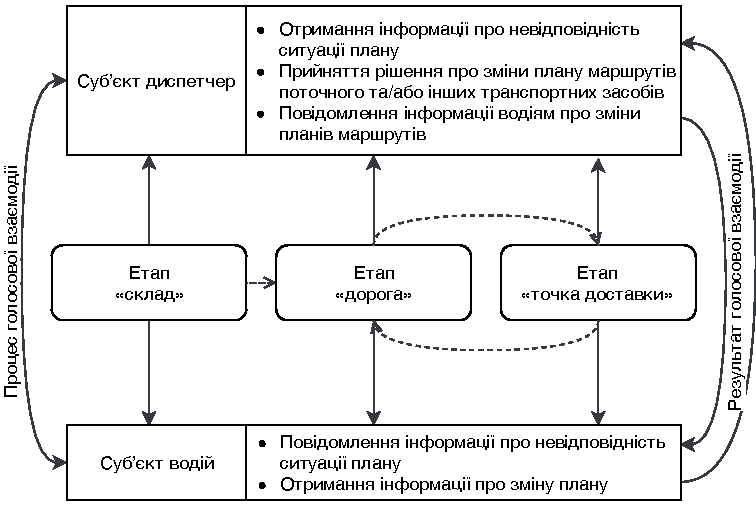
\includegraphics [width=\linewidth] {voice_interaction_schema}
	\caption{Схема голосової взаємодії субʼєктів дистрибуції}
	\label{img:voice_interaction_schema}
\end{figure}

Схему голосової взаємодії субʼєктів дистрибуції зображено на рис. \ref{img:voice_interaction_schema}. Вона складається з трьох етапів, з яких два останні можуть циклічно повторюватися за наявності в маршруті декількох точок доставки. Стрілками позначено процеси голосової взаємодії, які можуть розгортатися на кожному з етапів за наявної невідповідності плану та факту. У верхній та нижній частинах схеми показано принципові типи результатів голосової взаємодії для кожного з субʼєктів (диспетчера та водія). Ця логічна схема визначає принциповий алгоритм побудови дерева сценаріїв голосової взаємодії.

Другим важливим та перспективним напрямом, який дає змогу побудувати рефлекторну модель голосової взаємодії в задачах управління дистрибуцією, є застосування рефлекторних систем голосового управління. Ідея, яку покладено в основу цього підходу, полягає в тому, щоб замість переведення голосової інформації в текстову репрезентацію аналізувати безпосередньо інформаційну складову сказаного, визначаючи, яку з відомих реакцій потрібно виконати. Як вже цитувалося вище, «Традиційні системи розпізнавання мови засновані на принципі: „усна мова“ → „репрезентація мови набором лінгвістичних конструкцій“ → „розуміння мови“. На основі теорії несилової взаємодії може бути запропонована інша модель розпізнавання природної мови: „усна мова“ → „розрахунок несилової (інформаційної) взаємодії на реакції“ → „реакція (розуміння чи поведінка)“» \cite{Teslia_2014}.

Тобто, така система складатиметься з двох основних компонентів (рис. \ref{img:rgsu_concept}). Перший компонент --- розпізнавання мови. Це може бути будь-яка система переведення голосового сигналу в текстову репрезентацію --- як лексичну, так і фонетичну. В нашій роботі ми будемо використовувати фонетичну текстову репрезентацію, оскільки її створення не потребує наявності великих контекстно залежних словників, що є більш прийнятним для використання на мобільному пристрої з обмеженим доступом до мережі інтернет.

\begin{figure}
	\centering
	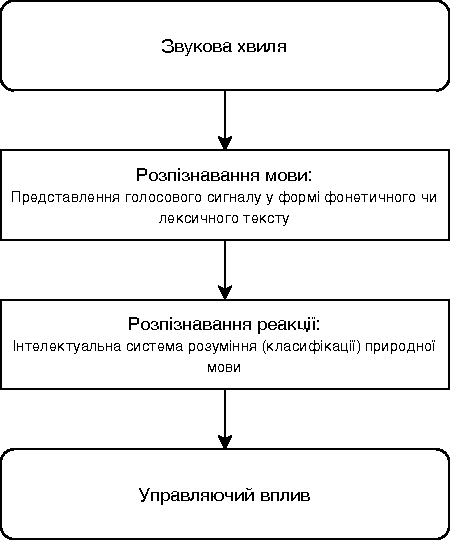
\includegraphics [width=.5\linewidth] {rgsu_concept}
	\caption{Схема узагальненої структури рефлекторних систем голосового управління}
	\label{img:rgsu_concept}
\end{figure}

Другий компонент --- розпізнавання реакції за розпізнаною  мовою. Концептуально це може бути будь-яка інтелектуальна система розуміння (класифікації) природної мови. В нашій роботі ми розглядатимемо метод інтелектуальних рефлекторних систем, оскільки його ефективність у роботі з фонетичним текстом вже доведено, і метод згорткових нейронних мереж, позаяк він показав гарні результати при роботі з лексичним текстом посимвольно, що є найбільш подібним до роботи з фонетичним текстом.

\section{Методи автоматизації руху автотранспорту в дистрибуції та параметри, що впливають на сценарії голосової взаємодії} \label{sect2_2}

Транспортна логістика --- це система організації доставки, тобто переміщення будь-яких матеріальних предметів або речовин з однієї точки в іншу за оптимальним маршрутом. Транспортна логістика є частиною процесів дистрибуції, курʼєрської доставки та інших транспортних систем, що мають в переліку своїх функцій перевезення вантажів. Важливим етапом у процесах транспортної логістики є так званий етап «останньої милі» --- останній етап доставки вантажу з розподільчого центру до клієнта. Він є найменш ефективним з усіх етапів ланцюга поставок і може коштувати до 28\% від усієї вартості доставки. \cite{Scott_2009}

Для транспортної логістики на етапі останньої милі надзвичайно важливим є планування маршрутів, а також моніторинг та диспетчеризація процесу доставки, оскільки якісно складений маршрут дає змогу зменшити транспортні витрати, а моніторинг --- підвищити рівень сервісу в реакціях на позапланові ситуації.

На жаль, сьогодні в більшості компаній України, що займаються перевезеннями, планування відбувається на досить примітивному рівні --- логісти визначають, який транспортний засіб який вантаж повезе, але не створюють конкретних маршрутів, залишаючи рішення про його вибір за водієм. Це повʼязано передусім з тим, що логісти розробляють планові маршрути вручну, без залучення автоматизованих систем. Друга причина (що, зауважимо, випливає з першої) полягає в тому, що логісти не можуть гарантувати принципову виконуваність маршрутів, оскільки орієнтуються здебільшого на масо-габаритні параметри, враховуючи часові вимоги лише частково. Це зумовлено тим, що масо-габаритні параметри можна порахувати сумарно незалежно від порядку обʼїзду точок доставки, тоді як часові параметри можна перевірити лише для конкретного маршруту, побудова і розрахунок якого без використання технічних засобів виходить за межі людських можливостей. Оскільки набір точок доставки для кожного окремого транспортного засобу не є гарантовано виконуваним, розраховувати маршрути окремих транспортних засобів немає сенсу --- потрібно вирішувати задачу в цілому для всіх точок доставки та машин, а це завдання відноситься до суттєво складнішого класу задач --- Vehicle Routing Problem (VRP).

Запровадження автоматичного розрахунку маршрутів має кілька суттєвих переваг. По-перше, це гарантованість принципової виконуваності маршрутів (без урахування позапланових ситуацій), по-друге --- підвищення рівня сервісу, адже, маючи конкретний маршрут з плановим часом прибуття, можемо повідомити його клієнту, скоротивши його час очікування. Наприклад, замовивши доставку з 15:00 до 18:00, клієнт буде позбавлений необхідності три години невідлучно <<сидіти на стільці>> в очікуванні, натомість матиме можливість  займатися своїми справами ,   відволікатися на інші завдання, лише час від часу перебуваючи в місці доставки. Якщо ж повідомимо клієнту орієнтовний час доставки (наприклад, з 17:00 по 17:30), то забезпечимо йому більшу свободу дій і знизимо ймовірність того, що саме в час прибуття доставки клієнт не зможе її прийняти вчасно, що призведе до затримки і подальшого відхилення від плану.

По-третє, наявність планового маршруту підвищить можливості моніторингу та своєчасного реагування на позапланові ситуації. Без планового маршруту за допомогою GPS-моніторингу можна лише побачити, де перебував транспортний засіб та де він зупинявся. Проте оскільки план, за яким рухається водій, невідомий, не буде зрозумілим, що саме означає зупинка: обслуговування точки доставки, чи відкладення обслуговування цієї точки на більш пізній час, ніж передбачено планом, чи водій тільки проїжджав повз, а зупинка --- це, наприклад, просто очікування дозволяючого рух сигналу світлофора тощо. Крім того, не маючи плану руху транспортного засобу, не можна спрогнозувати, чи встигає курʼєр обслуговувати всі точки доставки вчасно --- можливо побачити лише той факт, що якась із точок не відвідана, тоді як замовлений клієнтом час уже скінчився. Маючи ж плановий маршрут, можна в кожний момент спрогнозувати приблизний час прибуття на кожну з наступних точок з урахуванням можливого відставання та оцінити, чи не призведе це відставання до порушення замовлених клієнтом часових вікон у подальшому. Маючи таку інформацію, набагато легше вжити своєчасних дій --- повідомити водію про необхідність пришвидшити обслуговування точок або обговорити з клієнтом можливість перенесення часу доставки.

Не варто відкидати також і чинник можливої економії за рахунок покращення ефективності планових маршрутів завдяки запровадженню автоматизованого планування. Втім практика показує, що водій з досвідом роботи та/або добрим знанням ввіреної йому території здатен планувати свій маршрут досить якісно, іноді навіть перевершуючи якість автоматизованих рішень завдяки наявності більш детальної інформації про карту району. Однак автоматизоване планування може відвʼязати якість маршрутів від людського фактору --- рівня досвіду кожного конкретного водія.

Точне вирішення задачі маршрутизації транспортних засобів неможливе для задач такого рівня складності, з якими стикаються сучасні курʼєрські служби в містах-мегаполісах. Сучасні потреби у швидкості обрахунку здатні задовольнити далеко не всі евристичні алгоритми. Залежно від бізнес-процесів конкретної компанії та організації її системи обліку та контролю за помилками трапляються ситуації, коли остаточна інформація про наявні замовлення отримується вже після прибуття вантажу на розподільчий пункт, а отже часу на планування, завантаження та відправлення курʼєрів залишається дуже мало. Тому час розрахунку стандартної задачі доставки в 2--3 тисячі точок не може перевищувати 30--40 хвилин.

Основною ж проблемою впровадження систем побудови планових маршруті, як показує практика, є спротив інноваціям на рівні кінцевих виконавців. Водії, особливо якщо це наймані перевізники, а не співробітники компанії, відмовляються їхати по запропонованим програмою маршрутам. Перевізники не зацікавлені в глобальній оптимальності всіх маршрутів чи рівні сервісу кінцевого клієнта, якщо до цих параметрів не привʼязана їх матеріальна винагорода (платня). Зазвичай вони користуються маршрутним листом, сформованим лише за територіальними та масо-габаритними критеріями, до часових же обмежень кінцевих клієнтів ставляться доволі формально. Будь-які зміни звичних планів сприймаються ними дуже негативно, аж до саботування всього процесу. До того ж навіть в ідеально правильному рішенні може бути закладено необхідність заїзду на територію іншого водія для доставки в ті точки, які останній не встигне виконати, або необхідність доставки в точки, що знаходяться в районі, який водій погано знає. Це відбувається у випадках, коли навантаження в «рідному» районі водія в певний день є незначним і виконати його мужуть водії сусідніх районів, або коли в іншому місці, навпаки, навантаження велике і потребує залучення додаткових машин. Але більшість наявних евристик орієнтовані лише на сумарну вартість і можуть допускати подібного роду неоптимальності, навіть коли вони не зумовлені нагальною потребою.

Таким чином, постає необхідність розробки евристичного алгоритму, який би максимально враховував вимоги логістів та водіїв щодо оптимальності вибору точок з позиції кожного конкретного маршруту, при цьому не відкидаючи глобальну оптимальність при високій швидкості обрахунку.

Практика показує, що одним з найбільш визначальних вхідних параметрів, що може суттєво вплинути на результат планування та можливість його втілення у  реальність, є кількість часу, запланована на обслуговування в точці. Інші параметри визначені  достатньо чітко - масо-габаритні параметри відомі заздалегідь, дозволені часові вікна встановлює кінцевий клієнт. На сьогодні для визначення часу та відстані руху по дорозі між двома точками розроблено багато інструментів, які дають змогу прогнозувати результат з достатнім рівнем похибки на основі статистичних даних. Потрібне ж для визначення часу обслуговування точки достовірне джерело інформації наразі відсутнє: ані клієнт, ані водій, ані логіст не можуть його назвати. Найбільш поширеною помилкою є надання всім точкам однакового часу, наприклад, 10 чи 5  хвилин, незалежно від ваги та кількості вантажу, який необхідно доставити, або складності пошуку та підʼїзду до точки доставки тощо. Кращий варіант, який задіюється доволі часто, --- категоризація точок або конкретних замовлень та використання фіксованого часу на обслуговування для всіх замовлень в категорії. Найбільш правильним варіантом, що може принести суттєву економію транспортного ресурсу при побудові планових маршрутів, є статистичний аналіз історії часу обслуговування точок. Моделювати кількість часу, необхідного для виконання точки, потрібно, виходячи з таких параметрів: кількість часу, що витрачалася на обслуговування цієї та подбних до неї точок у минулому; водії, які їх  обслуговували, та тип машин, на яких вони при цьому працювали; вага, обʼєм та кількість вантажу, який було доставлено, тощо. Зазначимо, що питання вибору оптимального способу моделювання заслуговує на окреме дослідження.

Проте, перешкодою для здійснення подібного статистичного аналізу є проблема збору цих історичних даних. Досить точно час зупинки можна визначити за допомогою аналізу GPS-треку. Але цей метод має низку недоліків. По-перше, дані GPS мають похибку, яка може збільшуватись як залежно від якості апаратного забезпечення, так і залежно від території, що обслуговується. Відомо, наприклад, що в зонах висотної забудови GPS-сигнал істотно погіршується, а іноді навіть повністю втрачається. Це може згубно впливати на визначення часу зупинки або навіть на фіксацію самого факту зупинки взагалі. По-друге, навіть якщо відкинути похибку GPS як не суттєву або прийнятну, постає питання співвіднесення зупинок та точок доставки. У загальному випадку таке співвіднесення однозначно можливе тільки за умови, якщо в заданому радіусі є лише одна зупинка та одна точка доставки. У випадках, коли зупинка відбулася поза заданим радіусом, або коли біля точки зафіксовано кілька зупинок (у тому числі з причин хибної інтерпретації зупинки через похибки GPS), або, як це трапляється найчастіше, одна зупинка знаходиться близько до декількох точок, однозначно визначити, час якої із зупинок необхідно записати як час обслуговування точки, неможливо. У сучасному світі в містах-мегаполісах досить часто трапляються ситуації, коли необхідно зробити декілька доставок в один багатоквартирний будинок або сусідні будинки зі спільним двором. Це також унеможливлює автоматичний збір та аналіз великої частини статистичної інформації про час обслуговування точки на основі GPS-даних.

Отже дані GPS необхідно доповнити додатковою інформацією про те, коли водій-експедитор закінчив виконання однієї з точок в межах єдиної зупинки і почав виконання наступної. Практика показує, що спроби зобовʼязати водія в цей момент діставати телефон/планшет і вибирати в мобільному додатку експедитора відповідну команду, у кращому випадку призводять лише до того, що водій відмітить всі точки як виконані ще до або вже після виконання всіх доставок на зупинці, адже маніпуляції з планшетом потребують часу і вільних рук, які в цей момент у водія зазвичай бувають зайнятими. Вирішенням цієї проблеми може стати забезпечення водія/експедитора зручним інтерфейсом, який би не відволікав його від основного завдання. Таким нам видається голосовий інтерфейс, який сприйматиме команди про початок та завершення виконання доставки.


\section{Методи представлення дерева сценаріїв взаємодії з урахуванням неголосової інформації} \label{sect2_3}

Для представлення дерева сценаріїв найкраще підходить орієнтований граф, в якому вершини позначають стан системи та діалогові фрази, які озвучуватиме система, а ребра --- репліки (стимули), які можуть бути сприйняті системою в кожній конкретній вершині. Реакція на стимул може привести до переходу між станами, отже орієнтоване ребро проводиться від тієї вершини, в якій стимул може бути сприйнятий, до тієї, що позначає стан, в який система перейде, реагуючи на стимул. Таким чином, множина всіх ребер, що виходять з вершини, позначає перелік стимулів, між якими треба проводити розпізнання для стану, що відповідає цій вершині.

Зауважимо, що назва «дерево сценаріїв» використовується як сталий вираз, проте реально представити всю необхідну інформацію у вигляді дерева неможливо, адже переходи між станами неминуче приводять до утворення циклів. Тому для представлення такої інформації краще підходить граф.

На жаль такій схемі не вистачає повноти для представлення всіх можливих варіантів перебігу подій. По-перше, реакції системи не обмежуються переключенням станів (контекстів), що позначають доступний перелік стимулів, і відтворенням діалогових фраз. Основне корисне навантаження системи --- комунікація між водієм і диспетчером та керування процесом доставки, що потребує способу представлення інших реакцій на стимули, таких як відправлення певної інформації в диспетчерський центр, отримання інструкцій з диспетчерського центру, переключення внутрішніх змінних для можливості повідомити водію контекстно залежну інформацію про "поточну" точку доставки тощо.

По-друге, стимули, які можуть викликати певні реакції системи і, відповідно, переходи між станами, не обмежуються голосовими репліками, вимовленими водієм. Це можуть бути певні події, про які стало відомо з інших джерел інформації, як наприклад, команда від диспетчера на зміну маршруту, відміну чи перенесення точки доставки, або інформація з внутрішніх джерел даних --- датчиків GPS, датчиків роботи двигуна чи відкриття дверей. Використовуючи інформацію з внутрішніх датчиків, можна автоматизувати перехід між деякими станами, що підвищить зручність користування системою та до того ж зменшить кількість необхідних альтернатив для розпізнавання голосових стимулів.

Отже, для повноцінного опису ми маємо такі сутності:

\begin{itemize}
	\item \textbf{Контекст} або \textbf{Стан}, що задає перелік дозволених стимулів, які може сприйняти система, перебуваючи в цьому контексті;
	\item \textbf{Стимул} або \textbf{Подія} --- певна зовнішня інформація, що породжує відповідну реакцію. Стимул може бути голосовою реплікою від водія, командою, отриманою від диспетчера, або подією, породженою інформацією з внутрішніх датчиків, якщо вони доступні;
	\item \textbf{Реакція} системи відповідно до стимула. Рекцією може бути переключення контексту, відтворення діалогового голосового повідомлення, відправлення певної моніторингової інформації до диспетчерського центру,  переключення внутрішніх змінних тощо. Один стимул може породжувати декілька реакцій різних типів.
\end{itemize}


\section{Принципи побудови рефлекторної системи голосової взаємодії водія в системах диспетчерського контролю за рухом автотранспорту} \label{sect2_4}

\subsection{Застосування теорії несилової взаємодії як основи інтелектуальних рефлекторних систем} \label{subsect2_4_1}

Принципи побудови рефлекторних систем містяться у теорії несилової взаємодії. У роботі \cite{Teslia_2010} представлено компʼютерну модель ймовірнісної інтерпретації руху, згідно з якою єдина швидкість, з якою переміщуються обʼєкти, --- це швидкість світла у вакуумі, а очікувана швидкість дрейфу для будь-якого матеріального обʼєкта $V$ залежить лише від імовірності його зсуву в тому чи іншому напрямі і дорівнює:

\[
V=c\cdot(p-(1-p))=c\cdot(2p-1)
\]

\noindent
де $p$ --- ймовірність зсуву в напрямку руху; $c$ --- швидкість світла у вакуумі.

Згідно із зазначеною теорією кожен обʼєкт у межах компʼютерної моделі має певну власну визначеність щодо руху в одному чи іншому напрямку:

\[
p=\frac{i^+}{i^+ + i^-}
\]

\noindent
де $i^+$ --- розмір області визначення напрямку зміщення обʼєкта в напрямку руху; $i^-$ --- розмір області визначення напрямку зміщення обʼєкта проти напрямку руху.

Автором уведено величини визначеності та інформованості:

\begin{equation}
\label{eq:tnv3}
d=i^+ - i^-;
\end{equation}

\begin{equation}
\label{eq:tnv4}
i=i^+ + i^-,
\end{equation}

\noindent
де $d$ --- визначеність щодо зміщення в напрямку руху; $i$ --- інформованість щодо зміщення в напрямку руху.

Крім того, автор доводить, що для руху матеріальних обʼєктів ці величини компʼютерної моделі взаємозалежні і можуть бути обраховані за формулою:

\begin{equation}
\label{eq:tnv7}
i=\sqrt{d^2+1}.
\end{equation}

З приведених вище формул можна вивести наступні залежності \cite{Teslia_2010}:

\begin{equation}
\label{eq:tnv5}
p=0.5+\frac{d}{2i};
\end{equation}

\begin{equation}
\label{eq:tnv6}
V=\frac{dc}{i};
\end{equation}

\begin{equation}
\label{eq:tnv8}
d=\pm0.5\sqrt{\frac{p}{1-p}+\frac{1-p}{p}-2}.
\end{equation}

Якщо застосувати фізичні закони до інформаційно-ймовірнісної інтерпретації руху, отриманої з компʼютерної моделі, що лежить в основі теорії несилової взаємодії, можна вивести вирази для оперування визначеністю \cite{Teslia_2010_2}. З формули релятивістського додавання швидкостей отримано вираз для операції доповнення визначеності:

\begin{equation}
\label{eq:tnv9}
d_{xy}=d_yi_x-d_xi_y.
\end{equation}

Якщо відома визначеність та додаткова визначеність, можна визначити нову визначеність:

\begin{equation}
\label{eq:tnv10}
d_y=d_xi_{xy}+d_{xy}i_x.
\end{equation}

З інформаційної інтерпретації закону збереження імпульсу отримано вираз для складання визначеності:

\begin{equation}
\label{eq:tnv11}
d_\Sigma = \sum_{j=1}^N d_j.
\end{equation}


\subsection{Використання рефлекторного методу для побудови рефлекторної системи голосової взаємодії} \label{subsect2_4_2}

Принцип побудови рефлекторних систем спирається на гіпотезу, що не тільки рух матеріальних обʼєктів у розробленій компʼютерній моделі, а й усі системи різного рівня складності підкоряються формулам теорії несилової взаємодії . Так, наприклад, автор показує, що зазначені формули відповідають статистичним закономірностям у природно-мовному тексті \cite[розділ 8]{Teslia_2010}.

Для побудови інтелектуальних рефлекторних систем припускається залежність сумісної умовної ймовірності реакції від безумовної ймовірності реакції та часткових умовних ймовірностей реакції в цій системі, яка підкоряється фізичним законам збереження імпульсу компʼютерної моделі та може бути розрахована за наведеними вище формулами.

Алгоритмічною основою таких систем є рефлекторний метод обчислення адекватної реакції на сукупність різних слабоструктурованих вхідних впливів.

Якщо застосувати принципи теорії несилової взаємодії до рефлекторних систем голосової взаємодії водія та диспетчера, то під реакцією буде розумітися та чи інша команда з моделі голосової взаємодії, а під умовним впливом --- наявність того чи іншого набору N-грам фонем.

Схема реалізації цього методу включає етапи:

1. Розрахунок визначеності для інтелектуальної системи щодо всіх вхідних N-грам фонем і можливих голосових команд.

Аналогія визначеності реакцій і впливів у фізичній компʼютерній моделі --- це імпульс матеріальних обʼєктів. У такій моделі розглядаються обʼєкти, що впливають один на одного шляхом «зіткнення» та передачі власної інформації (імпульсу). Обʼєктам, що впливають, відповідають N-грами фонем, а обʼєктам, на які здійснюється вплив, --- можливі реакції (голосові команди). З (\ref{eq:tnv7}) та (\ref{eq:tnv8}) отримуємо:

\[
d(A_i)=\pm0.5\sqrt{\frac{p(A_i)}{1-p(A_i)}+\frac{1-p(A_i)}{p(A_i)}-2};
\]

\[
i(A_i)=\sqrt{d^2(A_i)+1};
\]

\[
d(A_i/B_j)=\pm0.5\sqrt{\frac{p(A_i/B_j)}{1-p(A_i/B_j)}+\frac{1-p(A_i/B_j)}{p(A_i/B_j)}-2};
\]

\[
i(A_i/B_j)=\sqrt{d^2(A_i/B_j)+1},
\]

\noindent
де: $p(A_i)$ --- безумовна ймовірність вибору команди $A_i$; $d(A_i)$ --- визначеність щодо команди $A_i$; $i(A_i)$ --- інформованість щодо команди $A_i$; $p(A_i/B_j)$ --- умовна ймовірність вибору команди $A_i$ (за наявності N-граму фонем $B_j$); $d(A_i/B_j)$ --- визначеність щодо команди $A_i$ за наявності N-граму фонем $B_j$; $i(A_i/B_j)$ --- інформованість щодо команди $A_i$ за наявності N-граму фонем $B_j$.

2. З інформаційно-ймовірнісної інтерпретації формули релятивістського додавання швидкостей (\ref{eq:tnv9}) отримано додаткову визначеність, що є в N-грамів фонем щодо голосових команд. Аналогією цього у фізичній компʼютерній моделі є швидкість руху обʼєктів, які здійснюють вплив, щодо обʼєктів, на які здійснюється вплив:

\[
\Delta d(A_i/B_j)=d(A_i/B_j)\cdot i(A_i)-d(A_i)\cdot i(A_i/B_j)
\]

\noindent
де $\Delta d(A_i/B_j)$ --- додаткова визначеність щодо команди $A_i$, яку надає наявність N-граму фонем $B_j$.

3. З інформаційно-ймовірнісної інтерпретації закону збереження імпульсу в компʼютерній моделі (\ref{eq:tnv11}) розраховано сумарний вплив на голосову команду, реакцію інтелектуальної системи, аналогом для якого у компʼютерній моделі виступає «удар» безлічі рухомих обʼєктів (відповідних дій, N-грамів фонем) по обʼєктах, відповідних реакціям (голосовим командам).

\[
d_\Sigma(A_i) = \sum_j \Delta d(A_i/B_j); \\
\]

\[
i_\Sigma(A_i) = \sqrt{\Delta d^2(A_i/B_j)+1},
\]

\noindent
де $d_\Sigma(A_i)$ --- сумарна додаткова визначеність щодо команди $A_i$ під впливом всіх N-грамів фонем $B_j$; $i_\Sigma(A_i)$ --- сумарна доповнювальна інформованість щодо команди $A_i$ під впливом всіх N-грамів фонем $B_j$.

4. Обчислюється нова визначеність голосової команди. Аналогом у фізичній компʼютерній моделі є нова швидкість руху після отриманого імпульсу під час зіткнення з обʼєктами, що здійснюють вплив:

\begin{equation}
\label{eq:ifron2}
d(A_i/B)=d_\Sigma(A_i)\cdot i(A_i)+d(A_i)\cdot i_\Sigma(A_i),
\end{equation}


\[
i(A_i/B) = \sqrt{d^2(A_i/B)+1},
\]

\noindent
де $d(A_i/B)$ --- нова визначеність щодо команди $A_i$ з урахуванням впливу всіх N-грамів фонем $B_j \in B$; $i(A_i/B)$ --- нова інформованість щодо команди $A_i$ з урахуванням впливу всіх N-грамів фонем $B_j \in B$.

5. За необхідності з (\ref{eq:tnv5}) можна обчислити сумісну умовну ймовірність команди $A_i$ (за наявності всіх N-грамів фонем $B_j \in B$):

\[
p(A_i/B)=0.5+\frac{d(A_i/B)}{2i(A_i/B)};
\]

\noindent
де $p(A_i/B)$ --- сумісна умовна ймовірність команди $A_i$ (за наявності всіх N-грамів фонем $B_j \in B$).

\section*{Висновки до розділу 2}
\addcontentsline{toc}{section}{Висновки до розділу 2}

1. Запропоновано концепцію створення системи автоматизації голосової взаємодії в задачах управління дистрибуцією, що має дві складові: (а) інтелектуальні рефлекторні системи голосового управління, що включають блок розпізнавання звукового сигналу та блок виділення його змісту; (б) модель сценаріїв взаємодії у процесах дистрибуції на трьох етапах доставки (завантаження на складі, дорога до точки доставки, розвантаження у точці доставки).

2. Розроблена система автоматичного розрахунку планових маршрутів та практика її використання забезпечили накопичення параметрів непередбачуваних ситуацій на плановому маршруті доставки, що впливають на створення сценаріїв голосової взаємодії.

3. Модель голосової взаємодії запропоновано будувати у вигляді орієнтованого графу, в якому вершини позначають стан системи та діалогові фрази, які озвучуватиме система, ребра – репліки (стимули), які можуть бути сприйняті системою в кожній конкретній вершині, а множина всіх ребер, що виходять з однієї вершини, позначатиме перелік стимулів розпізнання для її стану. У результаті для повноцінного опису запропоновано використовувати такі сутності: Контекст або Стан, Стимул або Подія, Реакція системи відповідно до стимулу.

4. Принципи побудови рефлекторних систем на основі теорії несилової взаємодії адаптовано для автоматизації голосової взаємодії в системах диспетчерського контролю за рухом автотранспорту.
